% arara: clean: {
% arara: --> extensions:
% arara: --> ['aux', 'log', 'nav', 'out',
% arara: --> 'pdf', 'snm', 'toc', 'vrb']
% arara: --> }
%! arara: lualatex: {
%! arara: --> shell: yes,
%! arara: --> draft: yes,
%! arara: --> interaction: batchmode
%! arara: --> }
%! arara: biber
% arara: lualatex: {
% arara: --> shell: yes,
% arara: --> draft: no,
% arara: --> interaction: batchmode
% arara: --> }
% arara: lualatex: {
% arara: --> shell: yes,
% arara: --> draft: no,
% arara: --> interaction: batchmode
% arara: --> }
% arara: clean: {
% arara: --> extensions:
% arara: --> ['aux', 'log', 'nav', 'out',
% arara: --> 'snm', 'toc', 'vrb']
% arara: --> }
\documentclass[
	8pt,
	professionalfonts,
	leqno,
	intlimits,
	c,
    aspectratio=1610,
]{beamer}
\usepackage{fontspec}
\usepackage{minted}
\usepackage{diffcoeff}

\setminted{breaklines=true}
\setminted[octave]{highlightcolor=yellow!50!white}
\setminted[cpp]{highlightcolor=yellow!50!white}
\setmonofont{Fira Code}[Contextuals=Alternate,Scale=MatchLowercase]

\usetheme{Madrid}
\usefonttheme[onlymath]{serif}
\setbeamertemplate{navigation symbols}{}

\title{1D Advection Equation}
\subtitle{Mimetic methods for solving PDEs and the MOLE library}
\author{Carlos Aznarán}

\begin{document}

\begin{frame}
    \maketitle
\end{frame}

\section{Objective of the study}

\begin{frame}
    \frametitle{\secname}
    \begin{block}{One-dimensional advection partial differential equation with constant velocity}
        Consider the following BVP/IVP for the advection equation
        with a Dirichlet boundary condition
        \begin{equation}\label{eq:bvpivp}
            \left\{
            \begin{aligned}
                \difcp{u}{t}\left(x,t\right)+
                c
                \difcp{u}{x}\left(x,t\right) & =
                f\left(x\right),             & x\in\left(a,b\right), t>0. \\
                u\left(a,t\right)            & =
                g\left(t\right),             & t>0.                       \\
                u\left(x,0\right)            & =
                u_{0}\left(x\right),         & x\in\left(a,b\right).
            \end{aligned}
            \right.
        \end{equation}

        The solution of~\eqref{eq:bvpivp} is given by
        \begin{equation*}
            u\left(x,t\right)=
            % \begin{cases}
            g\left(x-ct\right)+
            \int_{0}^{t}
            f\left(x-c\left(t-\theta\right)\right)\dl\theta. %& x-ct\geq a. \\
            % g\left(t-\frac{x-a}{c}\right),                   & x-ct<a.
            % \end{cases}
        \end{equation*}
    \end{block}

    \begin{example}[Non-homogeneous]
        \begin{equation*}
            \left\{
            \begin{aligned}
                \difcp{u}{t}\left(x,t\right)+
                c
                \difcp{u}{x}\left(x,t\right) & =
                1,                           & x\in\left(-1,1\right), t>0. \\
                u\left(-1,t\right)           & =
                0,                           & t>0.                        \\
                u\left(x,0\right)            & =
                x+1,                         & x\in\left(-1,1\right).
            \end{aligned}
            \right.
        \end{equation*}
        The solution is given by
        \begin{equation*}
            u\left(x,t\right)=
            \begin{cases}
                x-ct + 1 + t,                  & x-ct\geq -1. \\
                \frac{x+1}{c}+t-\frac{x+1}{c}, & x-ct<-1.
            \end{cases}
        \end{equation*}
    \end{example}
\end{frame}

\section{Application with the MOLE library}

\begin{frame}
    \frametitle{\secname}
    \begin{example}[Homogeneous]
        Let's consider the program~\href{https://raw.githubusercontent.com/carlosal1015/mole_examples/main/examples/octave/hyperbolic1D.m}{\mintinline{octave}|hyperbolic1D.m|} subject to the following configuration.
        \begin{equation*}
            \left\{
            \begin{aligned}
                \difcp{u}{t}\left(x,t\right)+
                \difcp{u}{x}\left(x,t\right) & =
                0,                           & x\in\left(0,1\right), t\in\left(0,1\right). \\
                u\left(0,t\right)            & =
                0,                           & t\in\left(0,1\right).                       \\
                u\left(x,0\right)            & =
                \sin\left(2\pi x\right),     & x\in\left(0,1\right).
            \end{aligned}
            \right.
        \end{equation*}
        The exact solution is given by
        \begin{equation*}
            u\left(x,t\right)=\sin\left(2\pi\left(x-at\right)\right).
        \end{equation*}
    \end{example}

    \begin{block}{Leapfrog scheme}
        \begin{equation*}
            u^{n+1}_{i}=
            u^{n}_{i}-
            \frac{c\Delta t}{\Delta x}
            \left(u^{n}_{i+1}-u^{n}_{i-1}\right)+
            \mathcal{O}\left(\Delta t^{2},\Delta x^{2}\right).
        \end{equation*}
    \end{block}

    \begin{alertblock}{CFL condition}
        Using von Neumann stability analysis it can be shown that the
        Leapfrog scheme is stable when
        \begin{equation*}
            \frac{\left|c\right|\Delta t}{\Delta x}\leq 1.
        \end{equation*}
    \end{alertblock}
\end{frame}

\section{Program with the MOLE library}

\begin{frame}
    \frametitle{\secname}
    \begin{listing}[H]
        \tiny
        \centering
        \inputminted[frame=single,framesep=10pt,linenos,firstline=1,lastline=37,highlightlines={17,18}]{octave}{../examples/octave/hyperbolic1D.m}
        % \caption{Program~\mintinline{octave}|hyperbolic1D.m|.}
        % \label{code:hyperbolic1D.m}
    \end{listing}
\end{frame}

\begin{frame}
    \frametitle{\secname}
    \begin{listing}[H]
        \tiny
        \centering
        \inputminted[frame=single,framesep=10pt,linenos,firstline=41,lastline=57,highlightlines={52-54}]{octave}{../examples/octave/hyperbolic1D.m}
    \end{listing}
\end{frame}

\section{Program's overview}

\begin{frame}
    \frametitle{\secname}
    \begin{itemize}
        \item The domain $\left[0,1\right]$ is divided with $50$ cells, $\Delta x=0.02$.
        \item The CFL condition ensure that stability for explicit schemes.
        \item We use the divergence operator of order $2$.
        \item We use the $1$D interpolation operator of order $2$
        \item The initial condition is $u\left(x,0\right)=\sin\left(2\pi x\right)$.
        \item We modify the first and last row for the divergence operator in order to impose the periodic boundary conditions.
        \item The spatial operator mixes the divergence and interpolation operators for approximate $-a\difcp{}{x}$.
        \item The factor $2$ fixes the scale in the staggered grid.
    \end{itemize}
\end{frame}

\section{Results}

\begin{frame}
    % \frametitle{\secname}
    \begin{figure}[H]
        \centering
        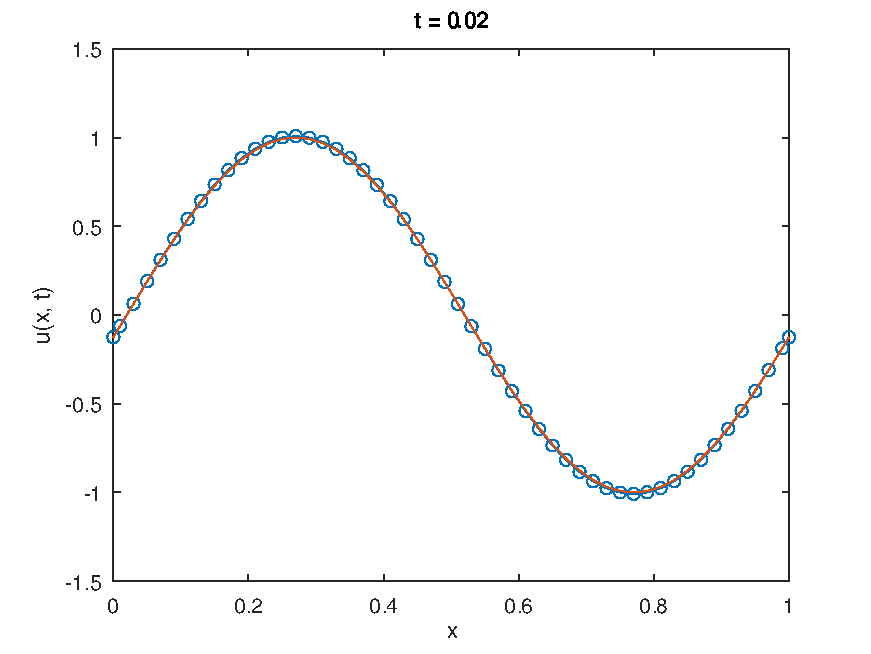
\includegraphics[width=.4\paperwidth]{../examples/octave/hyperbolic1D1.pdf}
        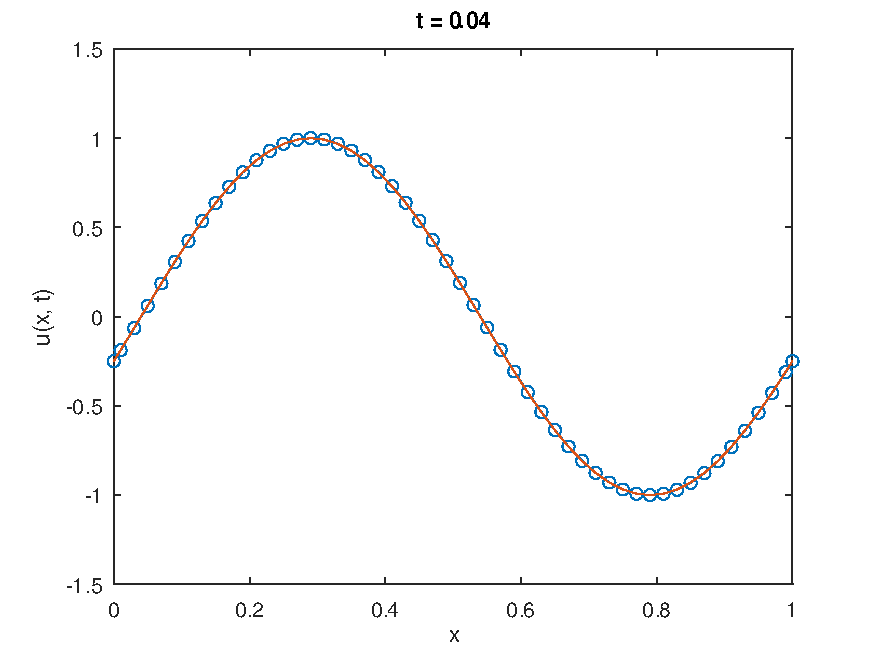
\includegraphics[width=.4\paperwidth]{../examples/octave/hyperbolic1D2.pdf}

        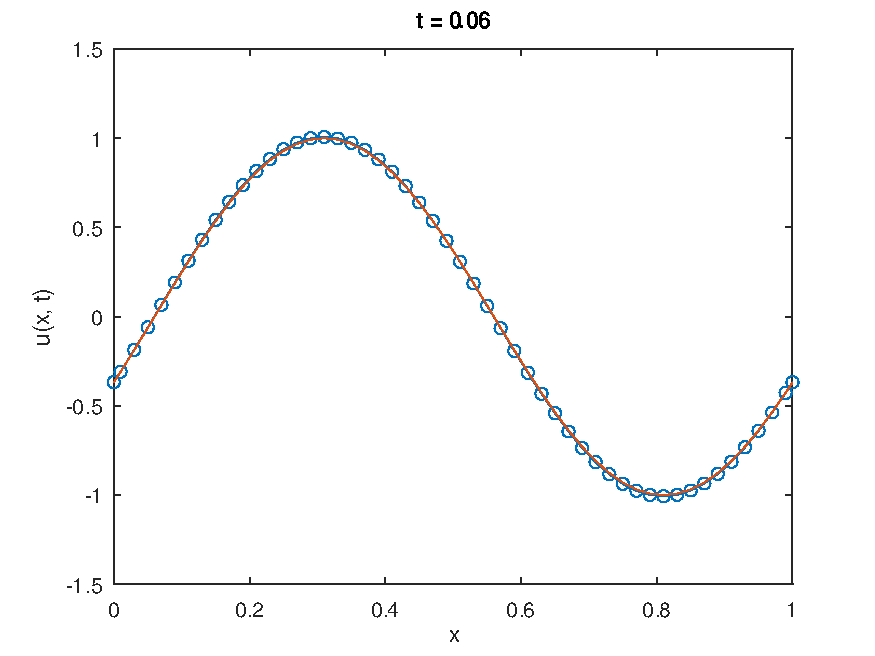
\includegraphics[width=.4\paperwidth]{../examples/octave/hyperbolic1D3.pdf}
        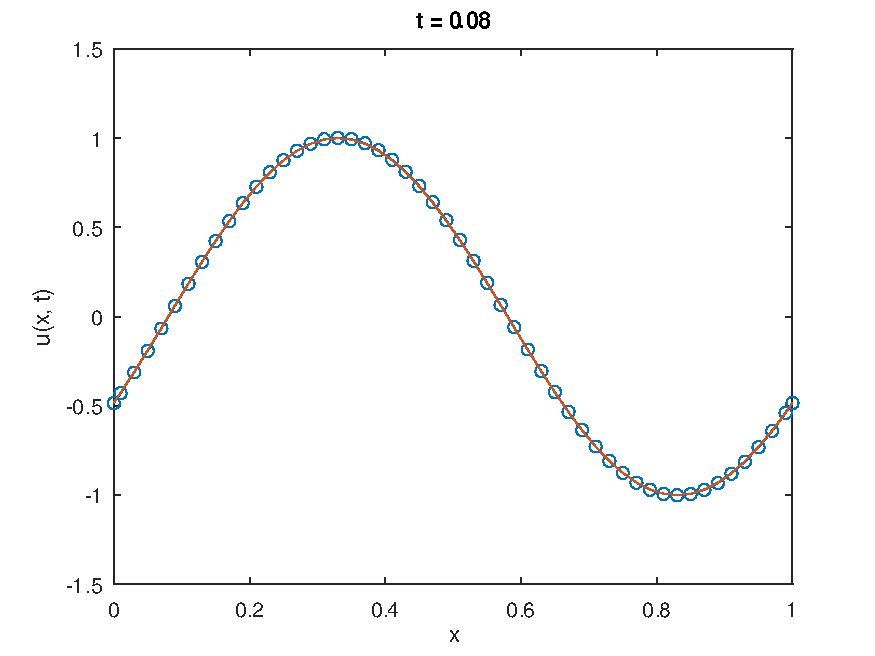
\includegraphics[width=.4\paperwidth]{../examples/octave/hyperbolic1D4.pdf}
    \end{figure}
\end{frame}

\begin{frame}
    % \frametitle{\secname}
    \begin{figure}[H]
        \centering
        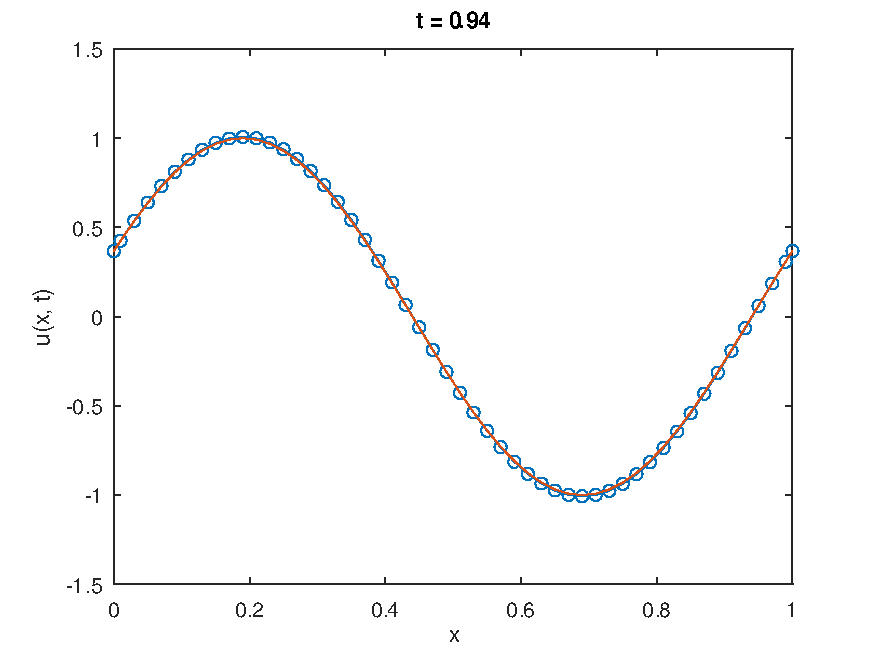
\includegraphics[width=.4\paperwidth]{../examples/octave/hyperbolic1D47.pdf}
        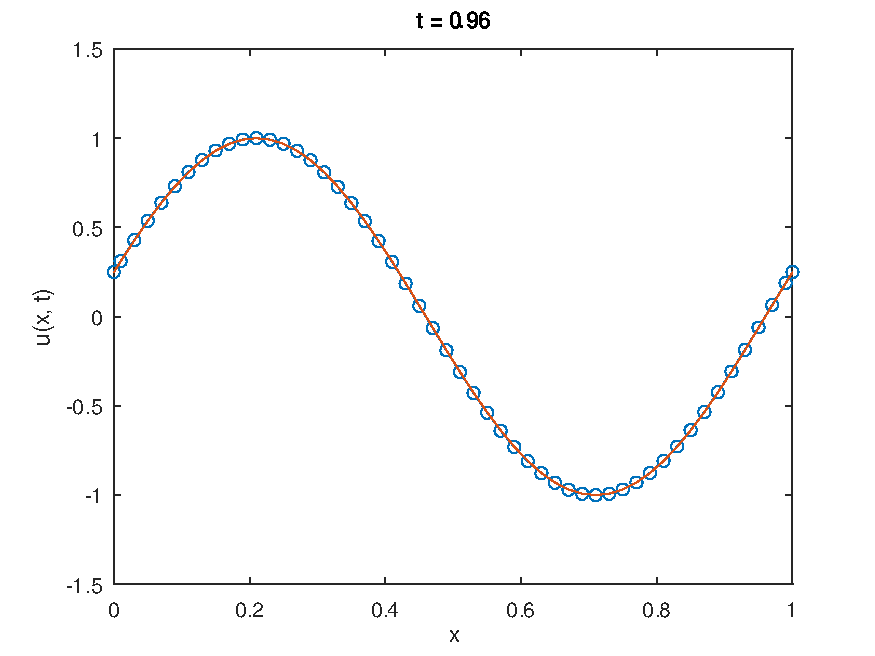
\includegraphics[width=.4\paperwidth]{../examples/octave/hyperbolic1D48.pdf}

        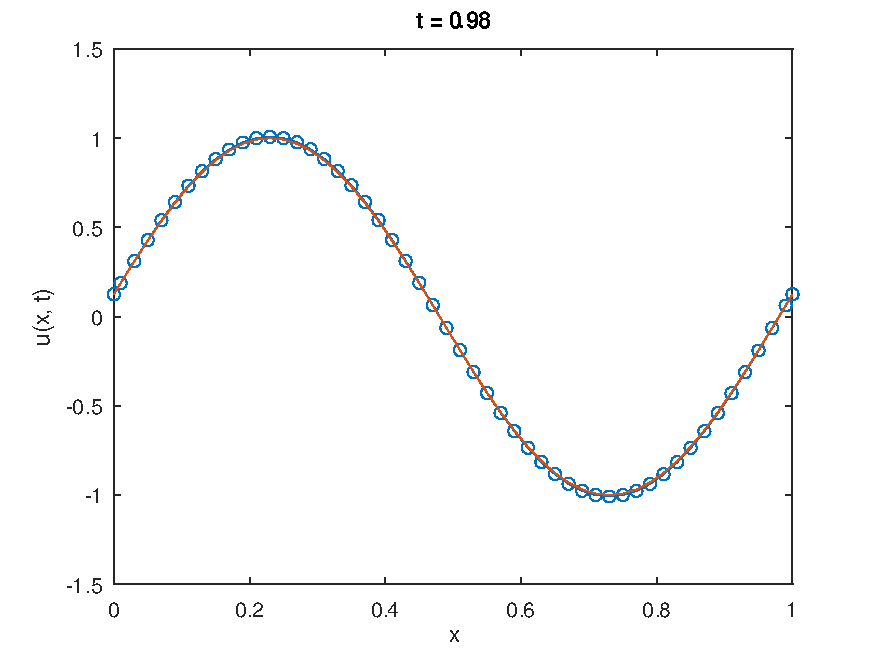
\includegraphics[width=.4\paperwidth]{../examples/octave/hyperbolic1D49.pdf}
        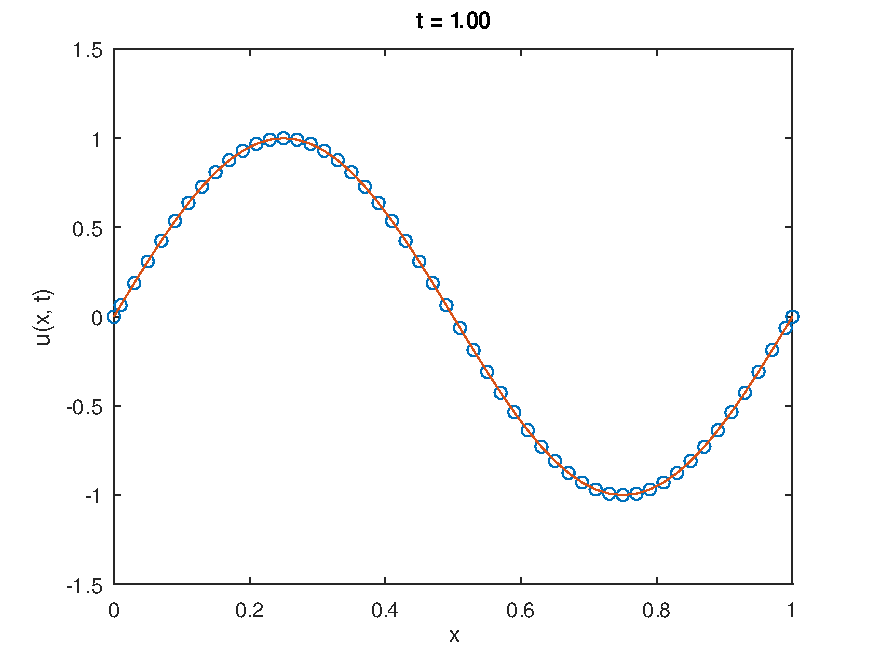
\includegraphics[width=.4\paperwidth]{../examples/octave/hyperbolic1D50.pdf}
    \end{figure}
\end{frame}

\end{document}